\chapter{User Guide}

\section{Code documentation for the library}

Documentation can be generated using the yard gem and then running the yard command. The command will output a \path{doc/} folder containing the documentation as a website.

\section{Getting the web application running}
\subsection{Installation}
One must only install the web application, as the library is automatically pulled when installing the requirements.

\begin{enumerate}
    \item Install dependencies: \texttt{\$ bundle install}
    \item Update database configuration:
    \begin{enumerate}
        \item Update \texttt{config/database.yml} with the MySQL details for the web application
        \item Update \texttt{config/initializers/assesor.rb} with the MySQL details for the web application
    \end{enumerate}
    \item Create web application database: \texttt{\$ bin/rake db:setup}
    \item Run database migrations: \texttt{\$ bin/rake db:migrate}
\end{enumerate}

\subsection{Starting the server}

The web application can be started using the command \texttt{bin/rails server}. The web application will be accessible on \texttt{localhost:3000}.

There are two defaults users created:
\begin{enumerate}
    \item Admin user:
    \begin{enumerate}
        \item Email: admin@example.com
        \item Password: test123
    \end{enumerate}
    \item Student user:
    \begin{enumerate}
        \item Email: student@example.com
        \item Password: test123
    \end{enumerate}
\end{enumerate}

\section{User management}
\Oldsubsection{Authentication}
A user must be authenticated at all time to access the application's functionality. Authentication is done on the path \texttt{/users/sign\_in}. A user will be automatically redirected to this page if he is not logged in. If a user uses a wrong email or password combination, he will see an error. The log in page is presented in figure \ref{fig:app:authentication}.

\begin{figure}[ht]
    \centering
    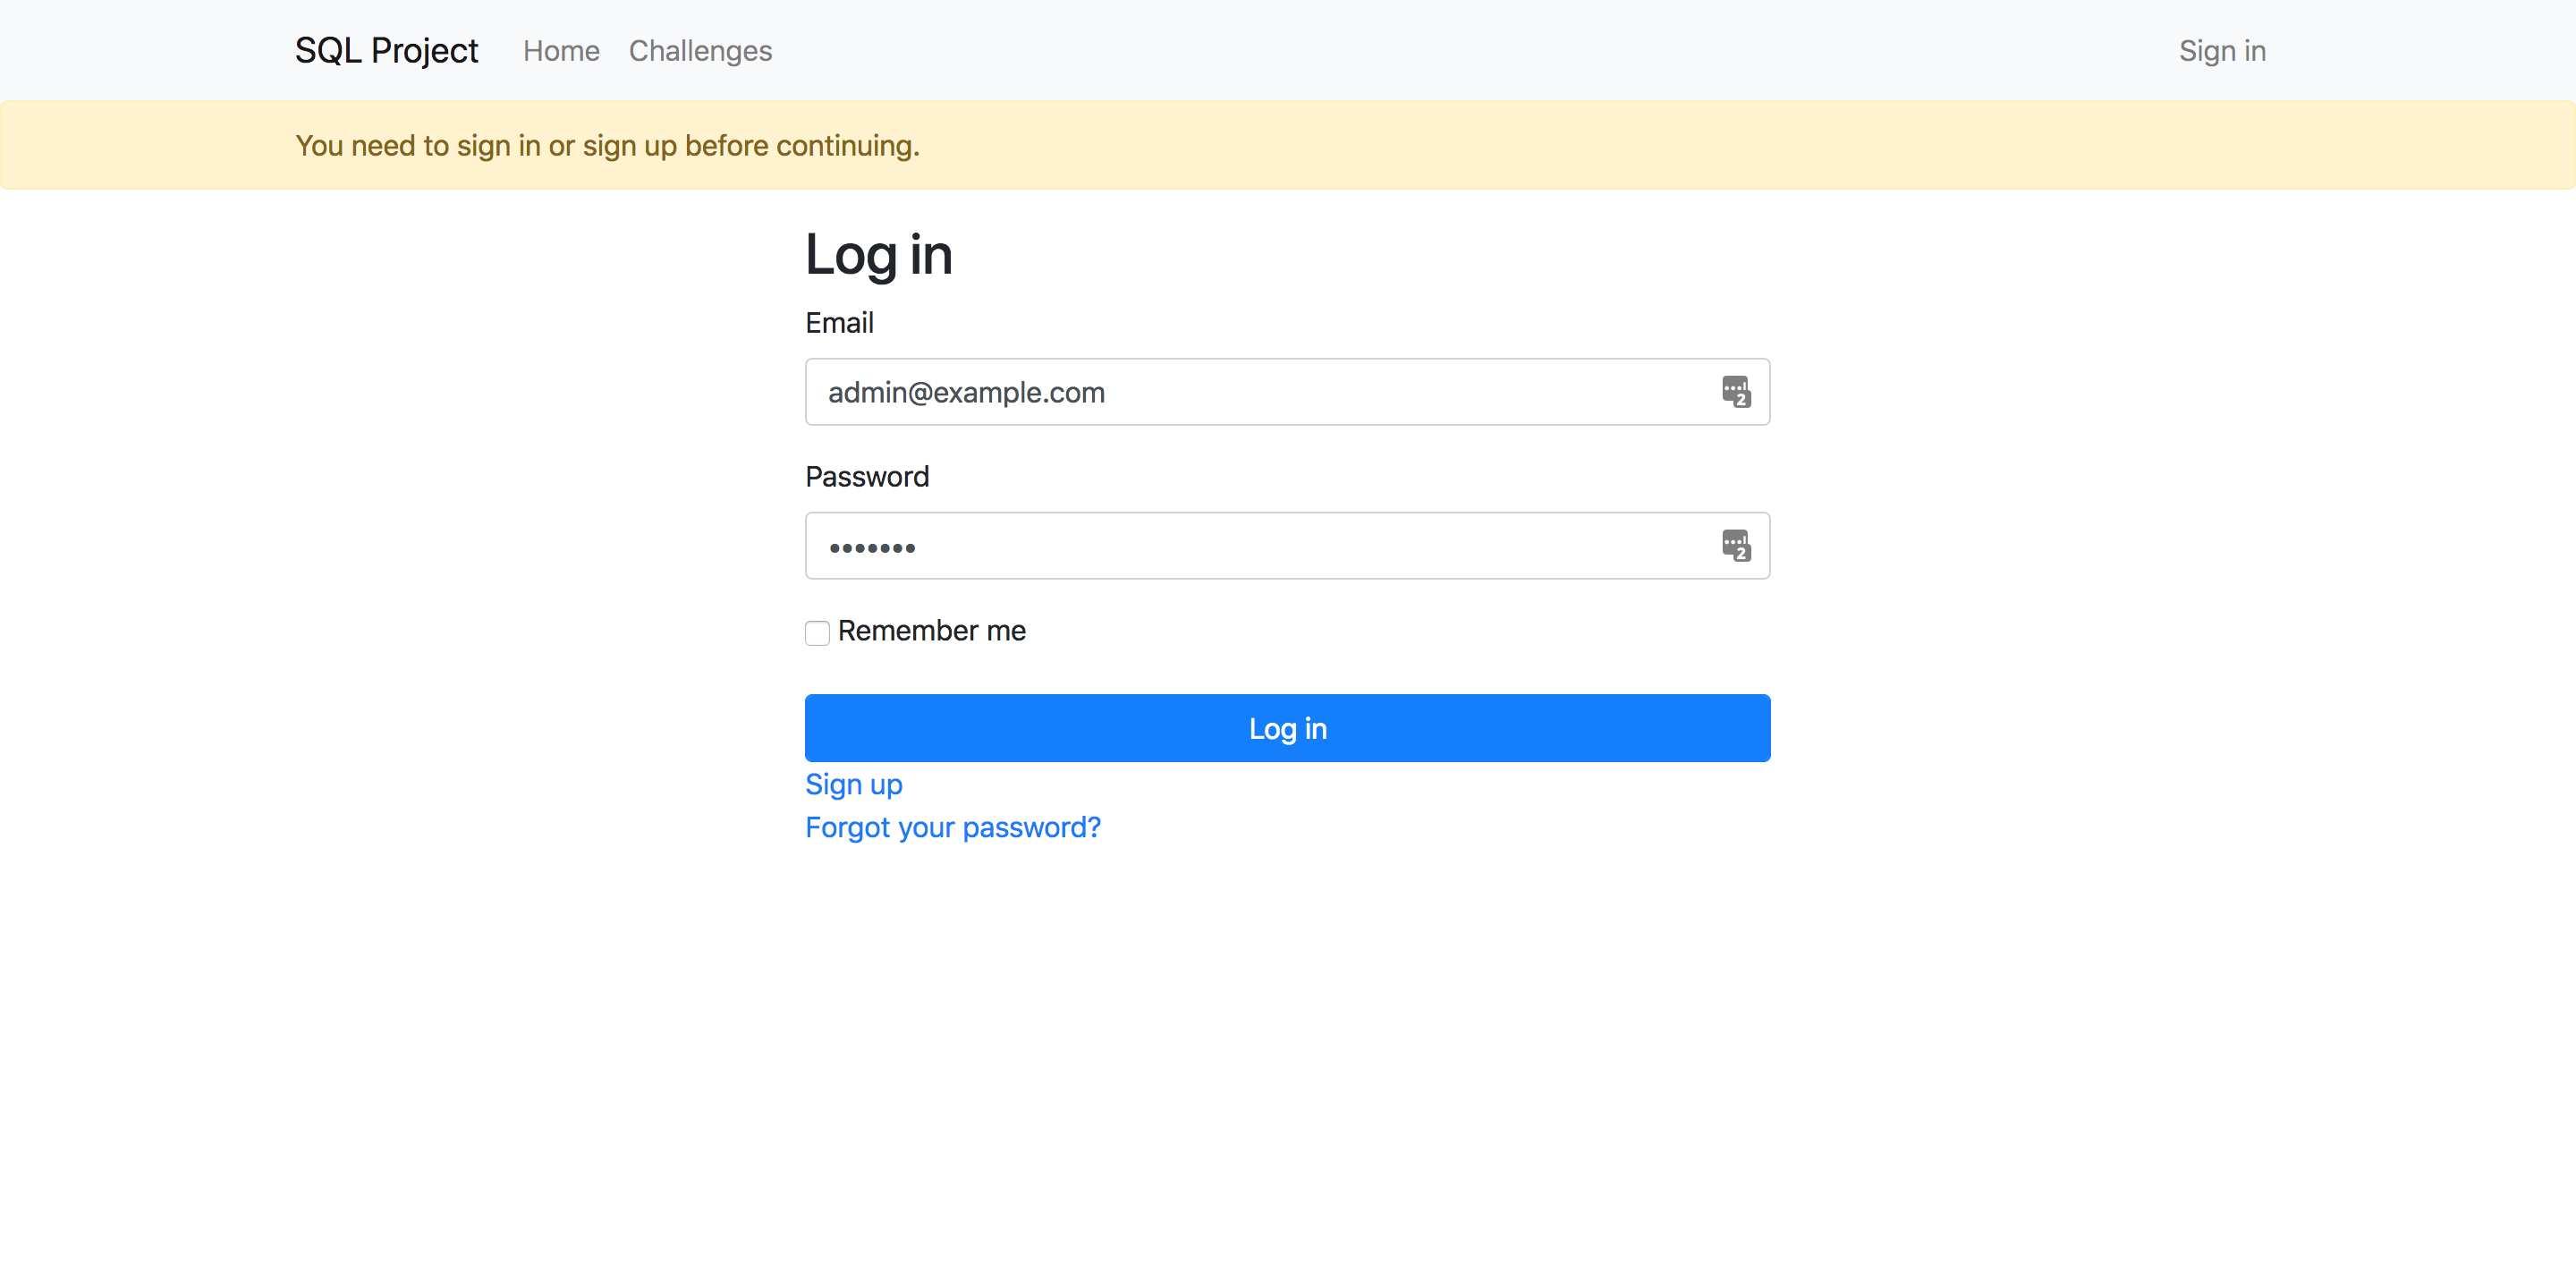
\includegraphics[width=\textwidth/4*3]{Appendices/authentication.png}
    \caption{Authentication screen}
    \label{fig:app:authentication}
\end{figure}

\Oldsubsection{Creating new user}
A new user can be created on the web application on path \texttt{/users/sign\_up} or by clicking the sing up button from the login page. Users are automatically marked as students. If a user uses a wrong email or password combination, he will see an error. An example of the sign-up page with errors is presented in figure \ref{fig:app:newuser}.

\begin{figure}[ht]
    \centering
    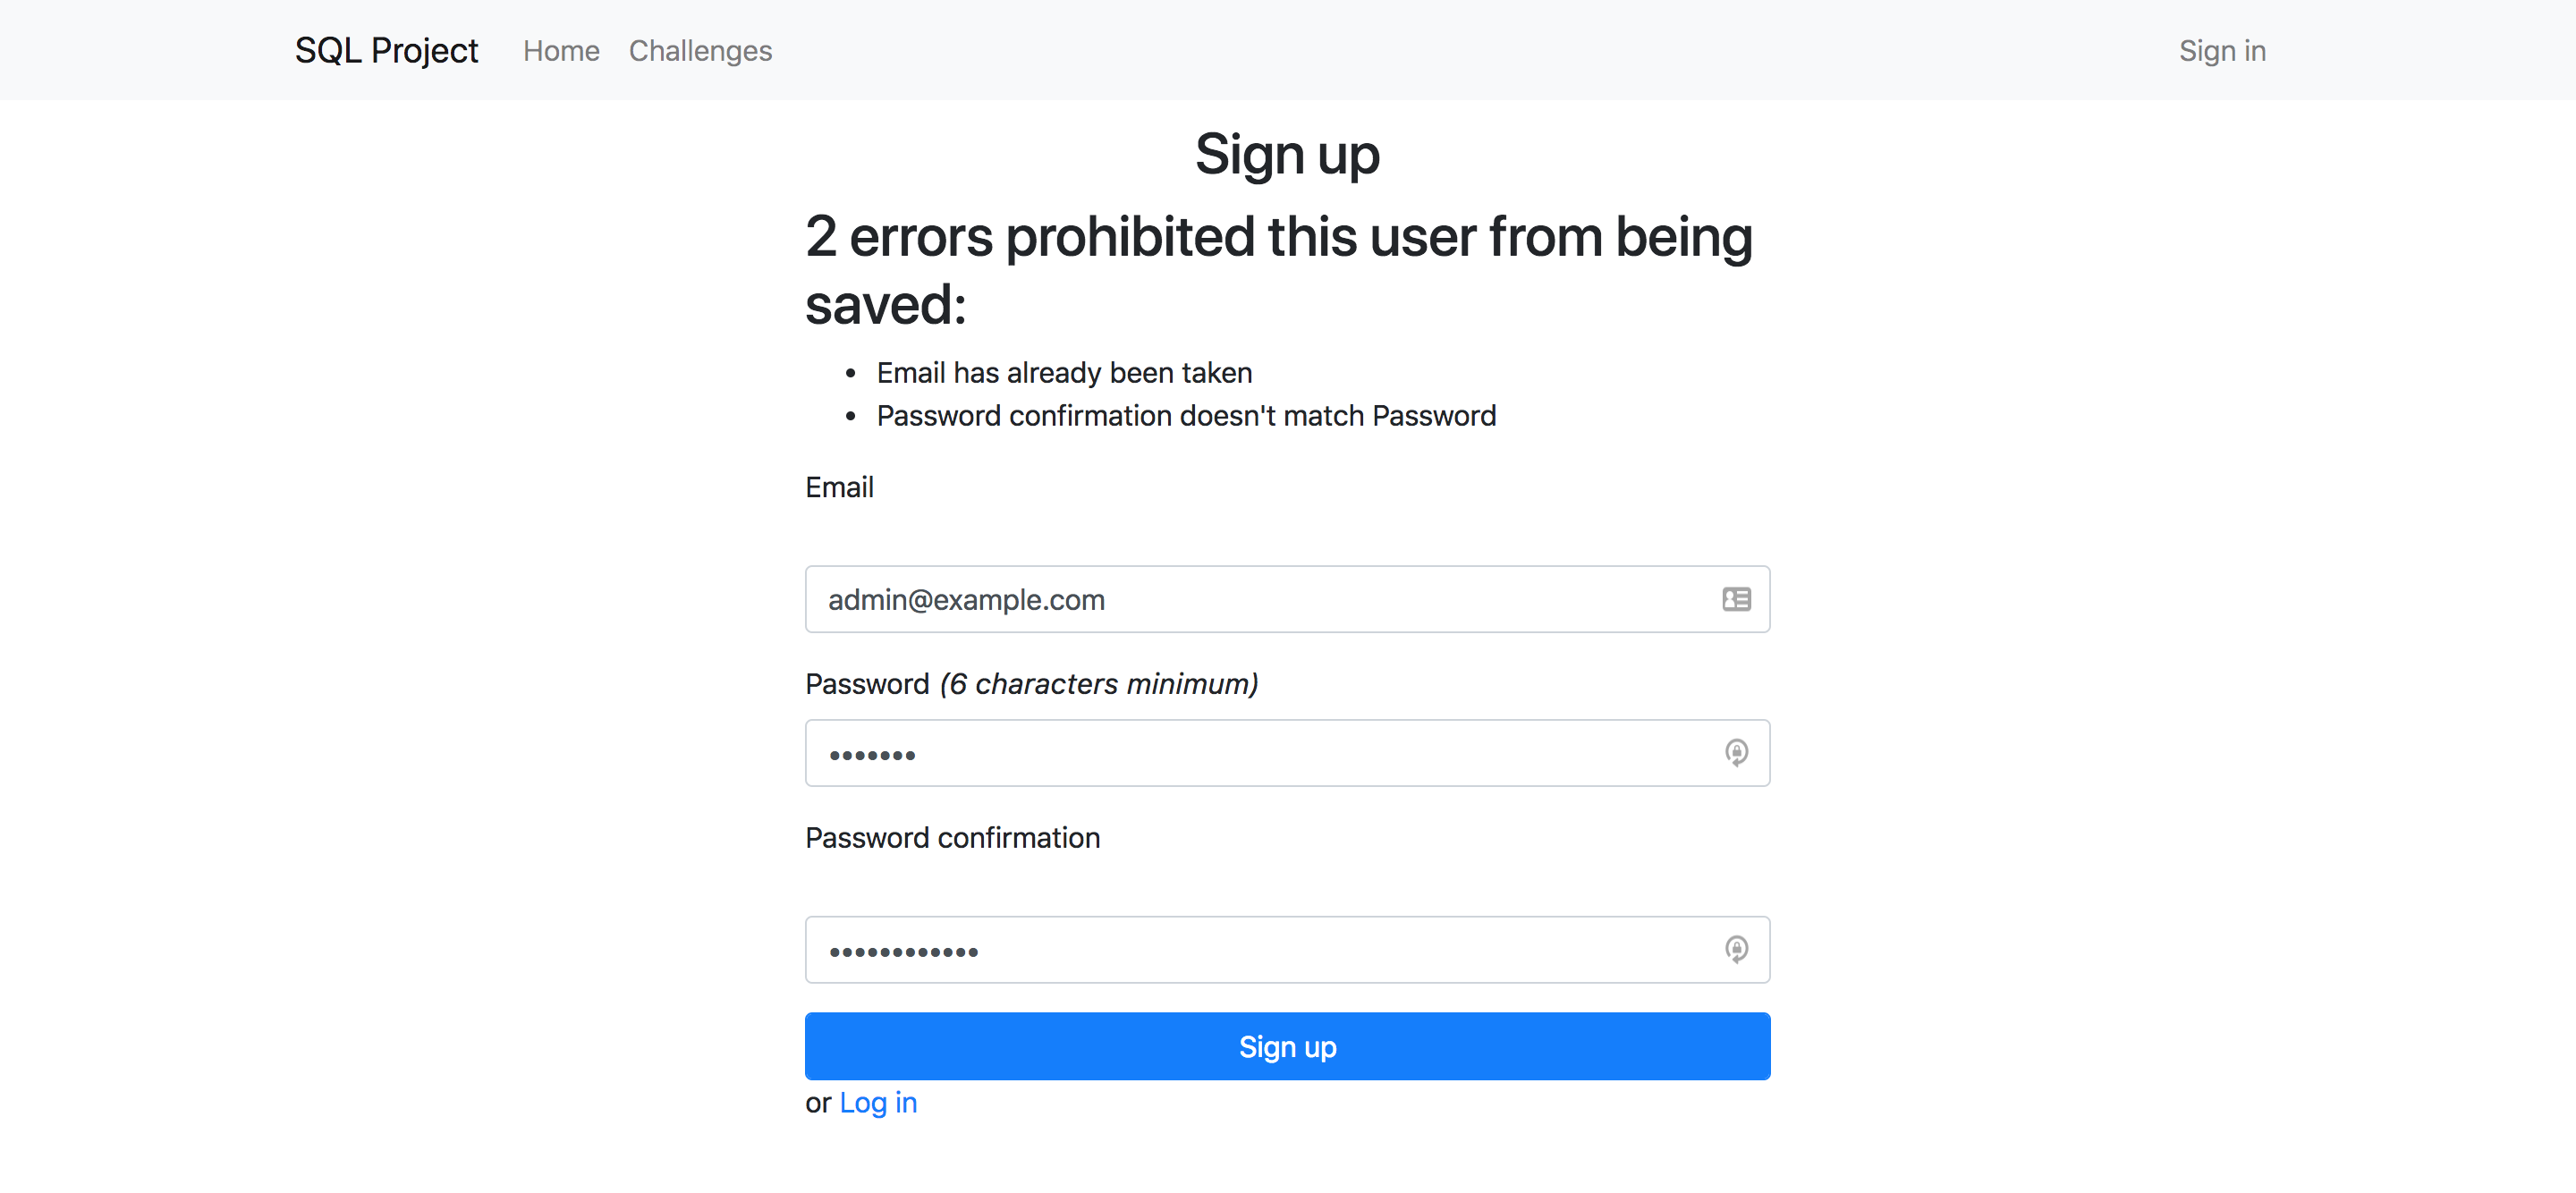
\includegraphics[width=\textwidth/4*3]{Appendices/signup.png}
    \caption{Sign-up screen}
    \label{fig:app:newuser}
\end{figure}

\Oldsubsection{Editing user details}
A user can change his details (email and password) on \texttt{/users/edit} or by clicking the Edit Profile in the navigation bar. The navigation bar link is presented in figure \ref{fig:app:editusernavbar} On this page, he can also delete his account. A photo of the page is included in figure \ref{fig:app:edituser}.

\begin{figure}[ht]
    \centering
    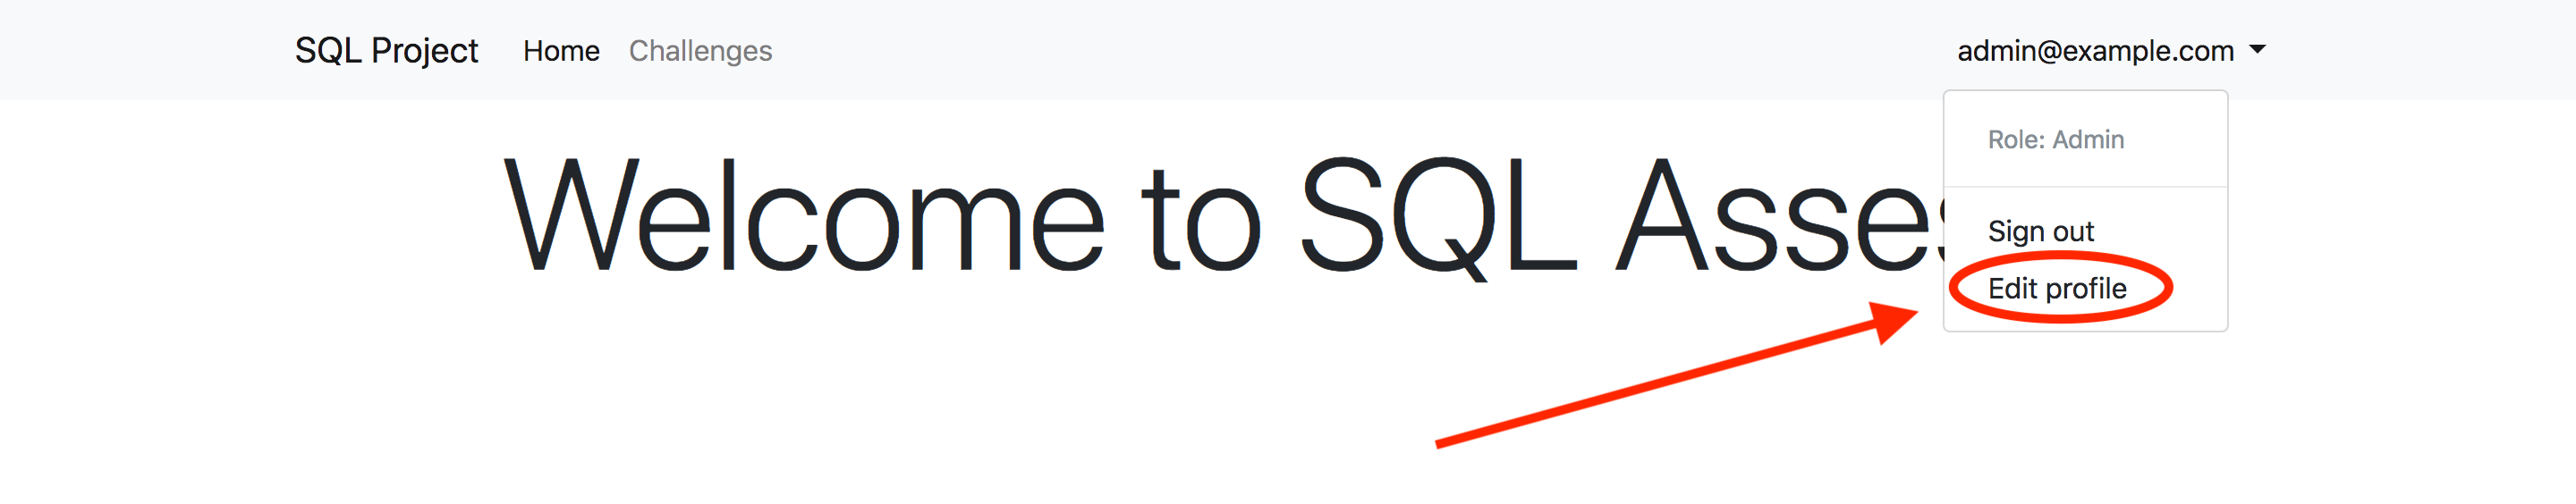
\includegraphics[width=\textwidth/4*3]{Appendices/editlinknavbar.png}
    \caption{Navigation bar link for edit user}
    \label{fig:app:editusernavbar}
\end{figure}

\begin{figure}[ht]
    \centering
    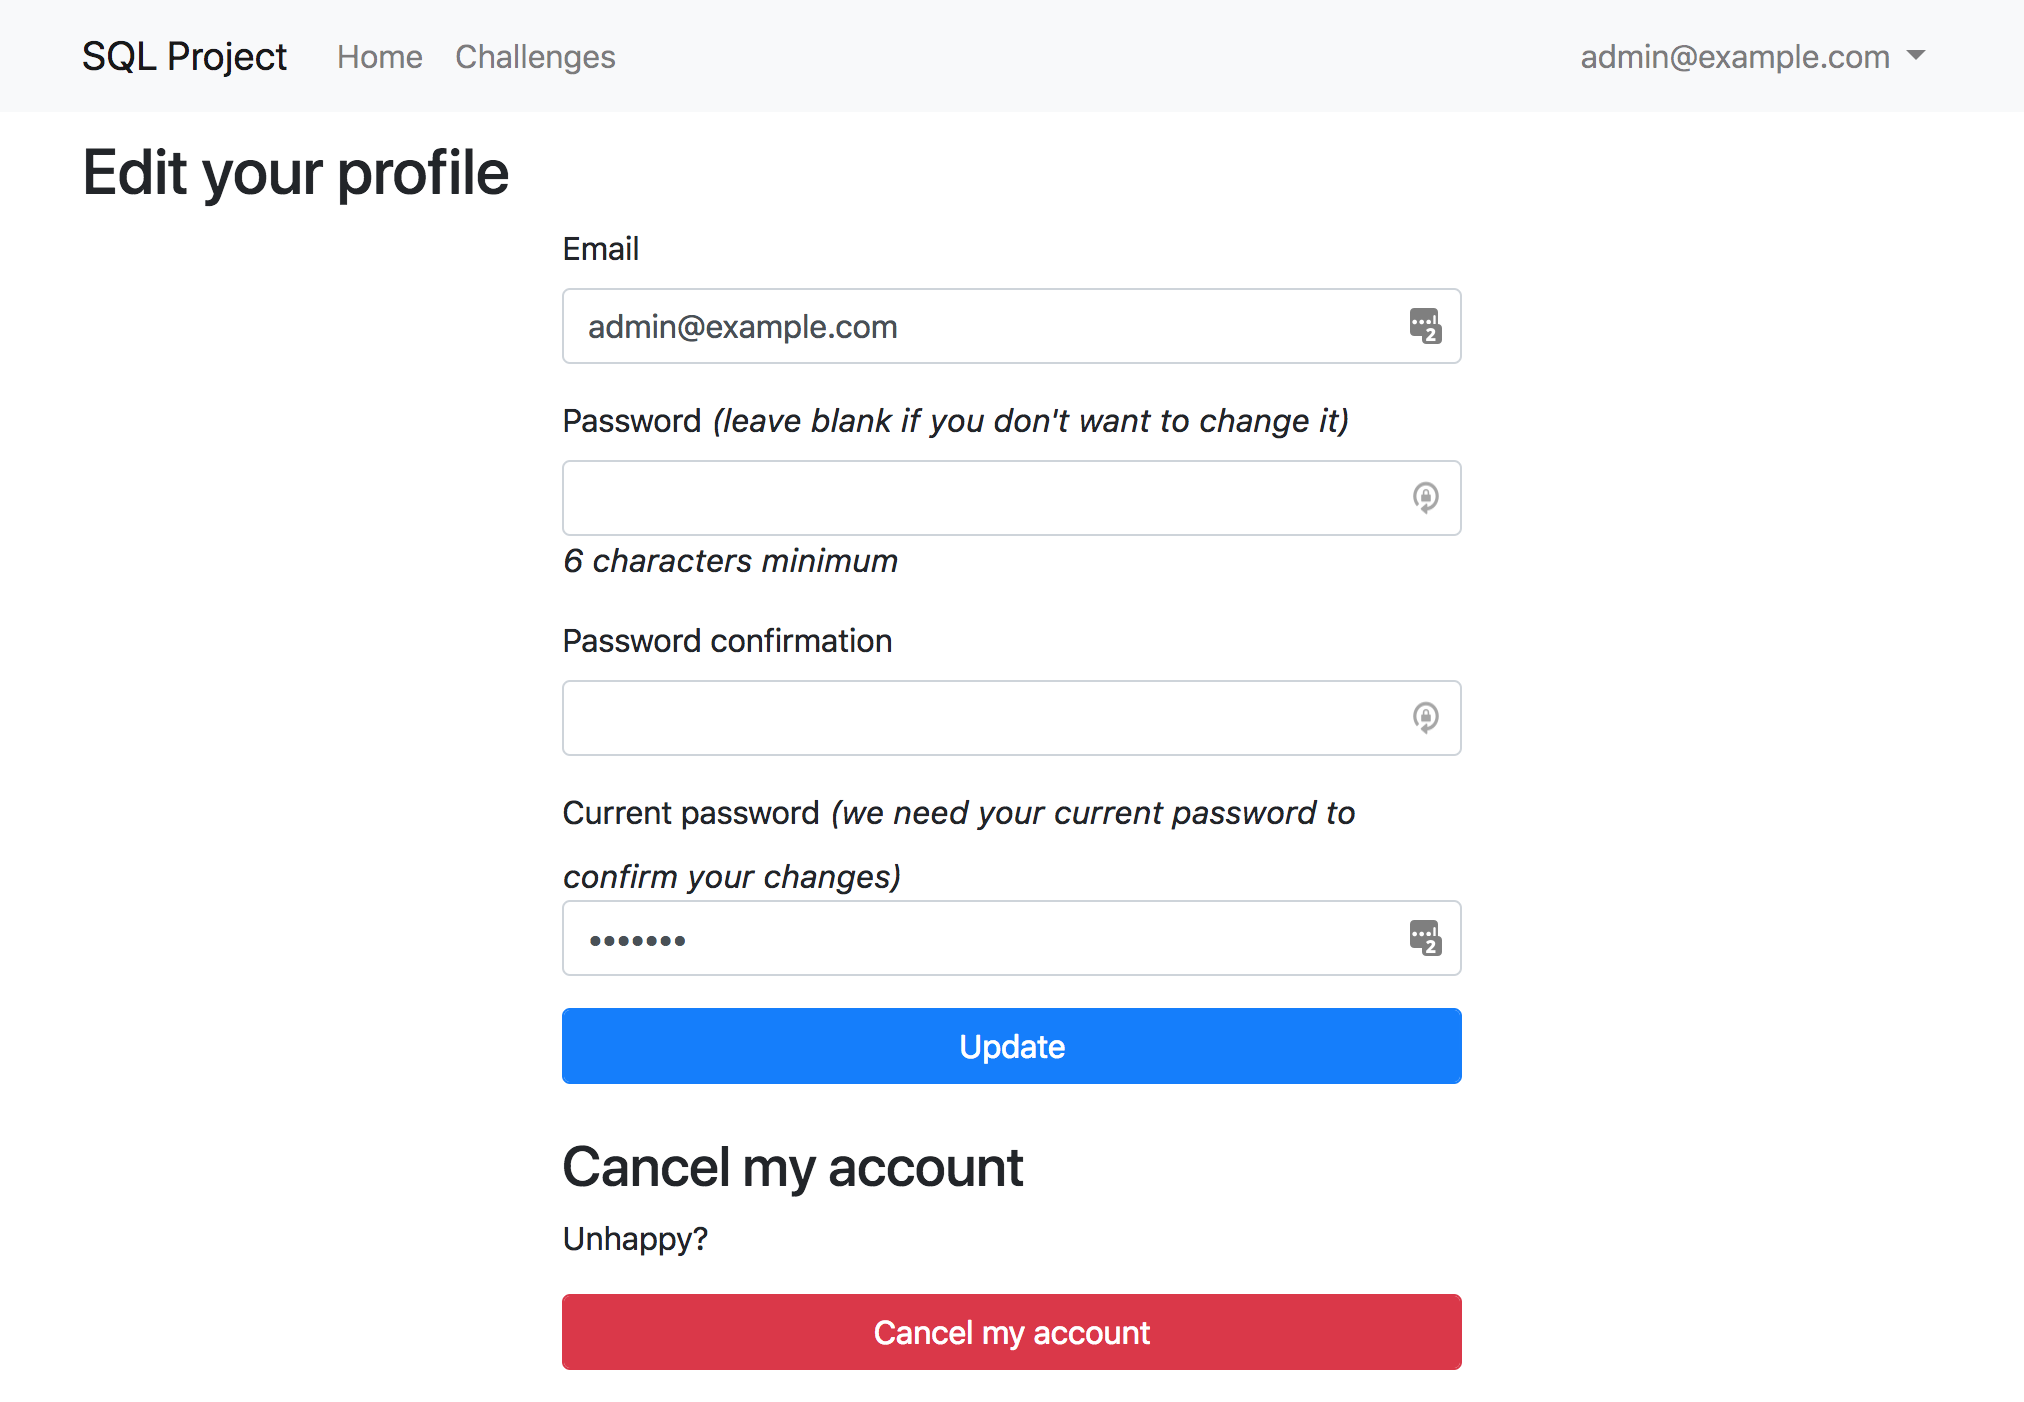
\includegraphics[width=\textwidth/4*3]{Appendices/edituser.png}
    \caption{Edit user page}
    \label{fig:app:edituser}
\end{figure}

\Oldsubsection{Sign-out}
Signing out is done from the navigation bar. Figure \ref{fig:app:signout} presents the location of the button.

\begin{figure}[ht]
    \centering
    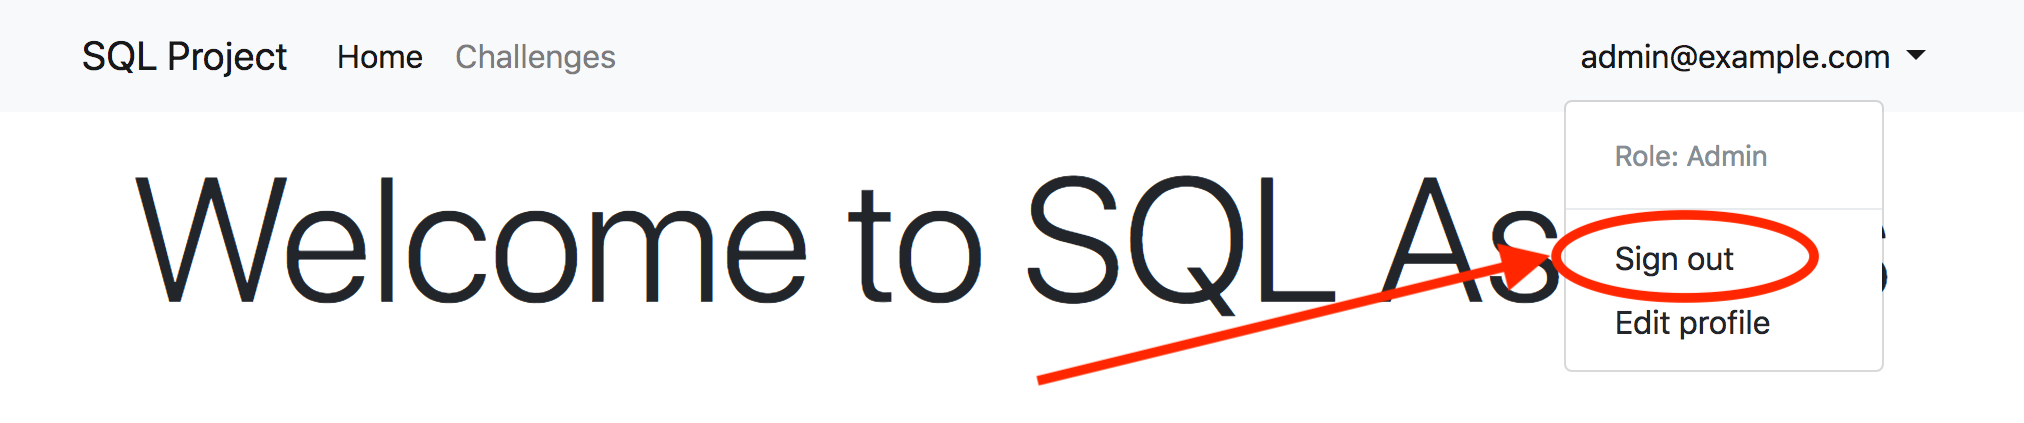
\includegraphics[width=\textwidth/4*3]{Appendices/signout.png}
    \caption{Sign out button}
    \label{fig:app:signout}
\end{figure}

\section{Challenge management}
To create a challenge, the current user must be an admin. To create a challenge, one must go to \texttt{/challenges/new}, or click \textit{Challenges} in the navigation bar, and then click \textit{Create new Challenge} button. The screen is presented in figure \ref{fig:app:new_challenge}.

The new challenge page requires 5 pieces of information:
\begin{enumerate}
    \item A title for the challenge
    \item The content or the challenge - or the body of the challenge
    \item SQL query for schema creation
    \item SQL query for data insertion
    \item The correct SQL query for the challenge
\end{enumerate}

The input for the SQL fields is a code editor that provides code syntax highlighting.

Any errors that might be encountered are shown to the user.
\begin{figure}[ht]
    \centering
    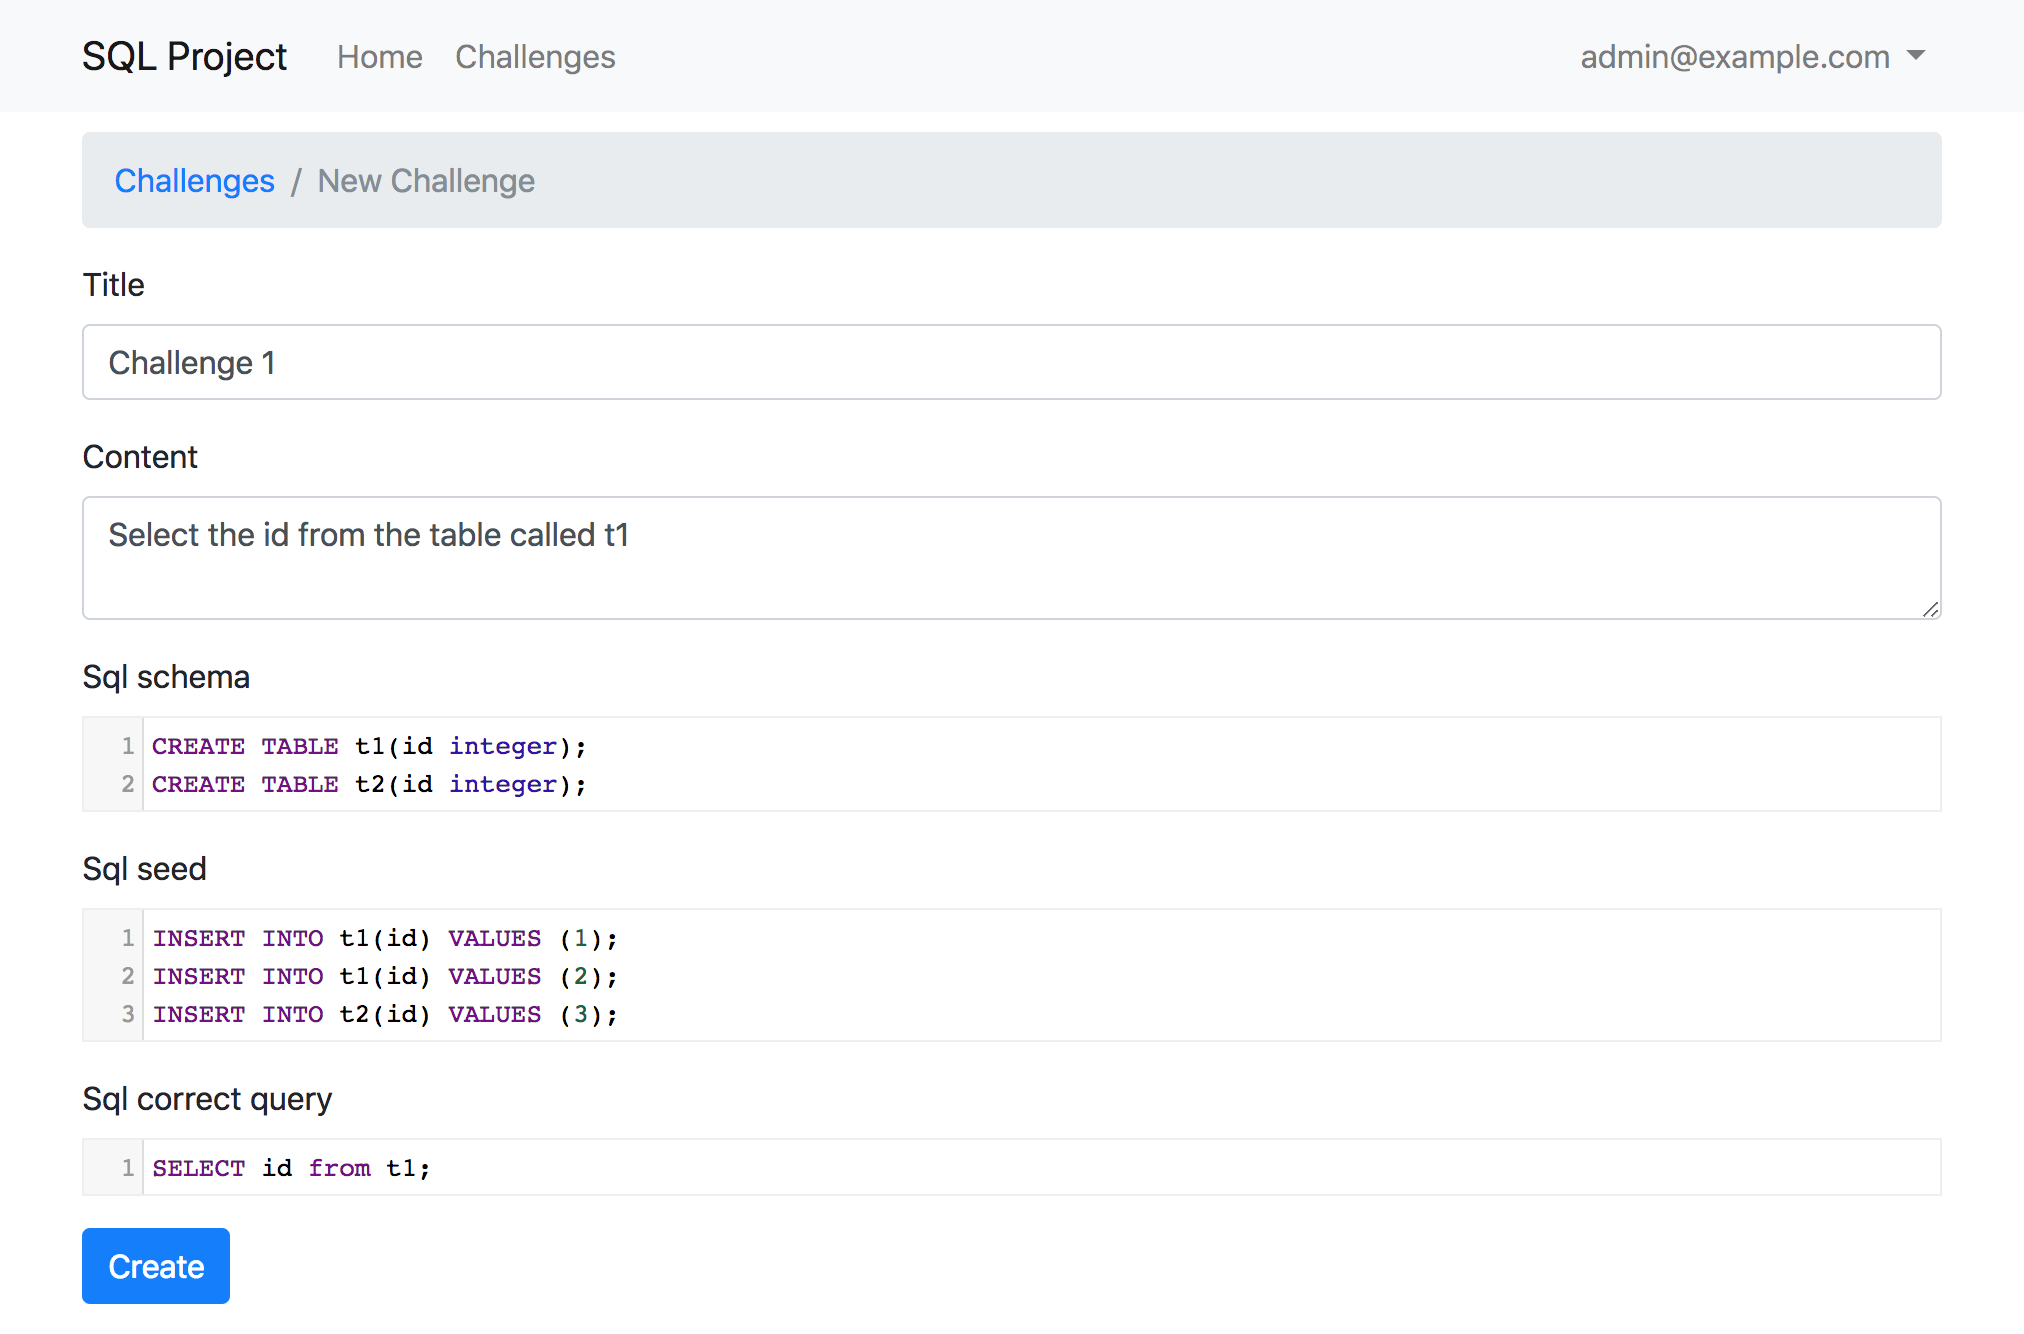
\includegraphics[width=\textwidth/4*3]{Appendices/new_challenge.png}
    \caption{New challenge form}
    \label{fig:app:new_challenge}
\end{figure}

Once the challenge has been saved, the user is redirect to the challenge page which contains all the details about the challenge (schema and existing fields). A screen-shot of the page is show in figure \ref{fig:app:challengeadmin}.

\begin{figure}[ht]
    \centering
    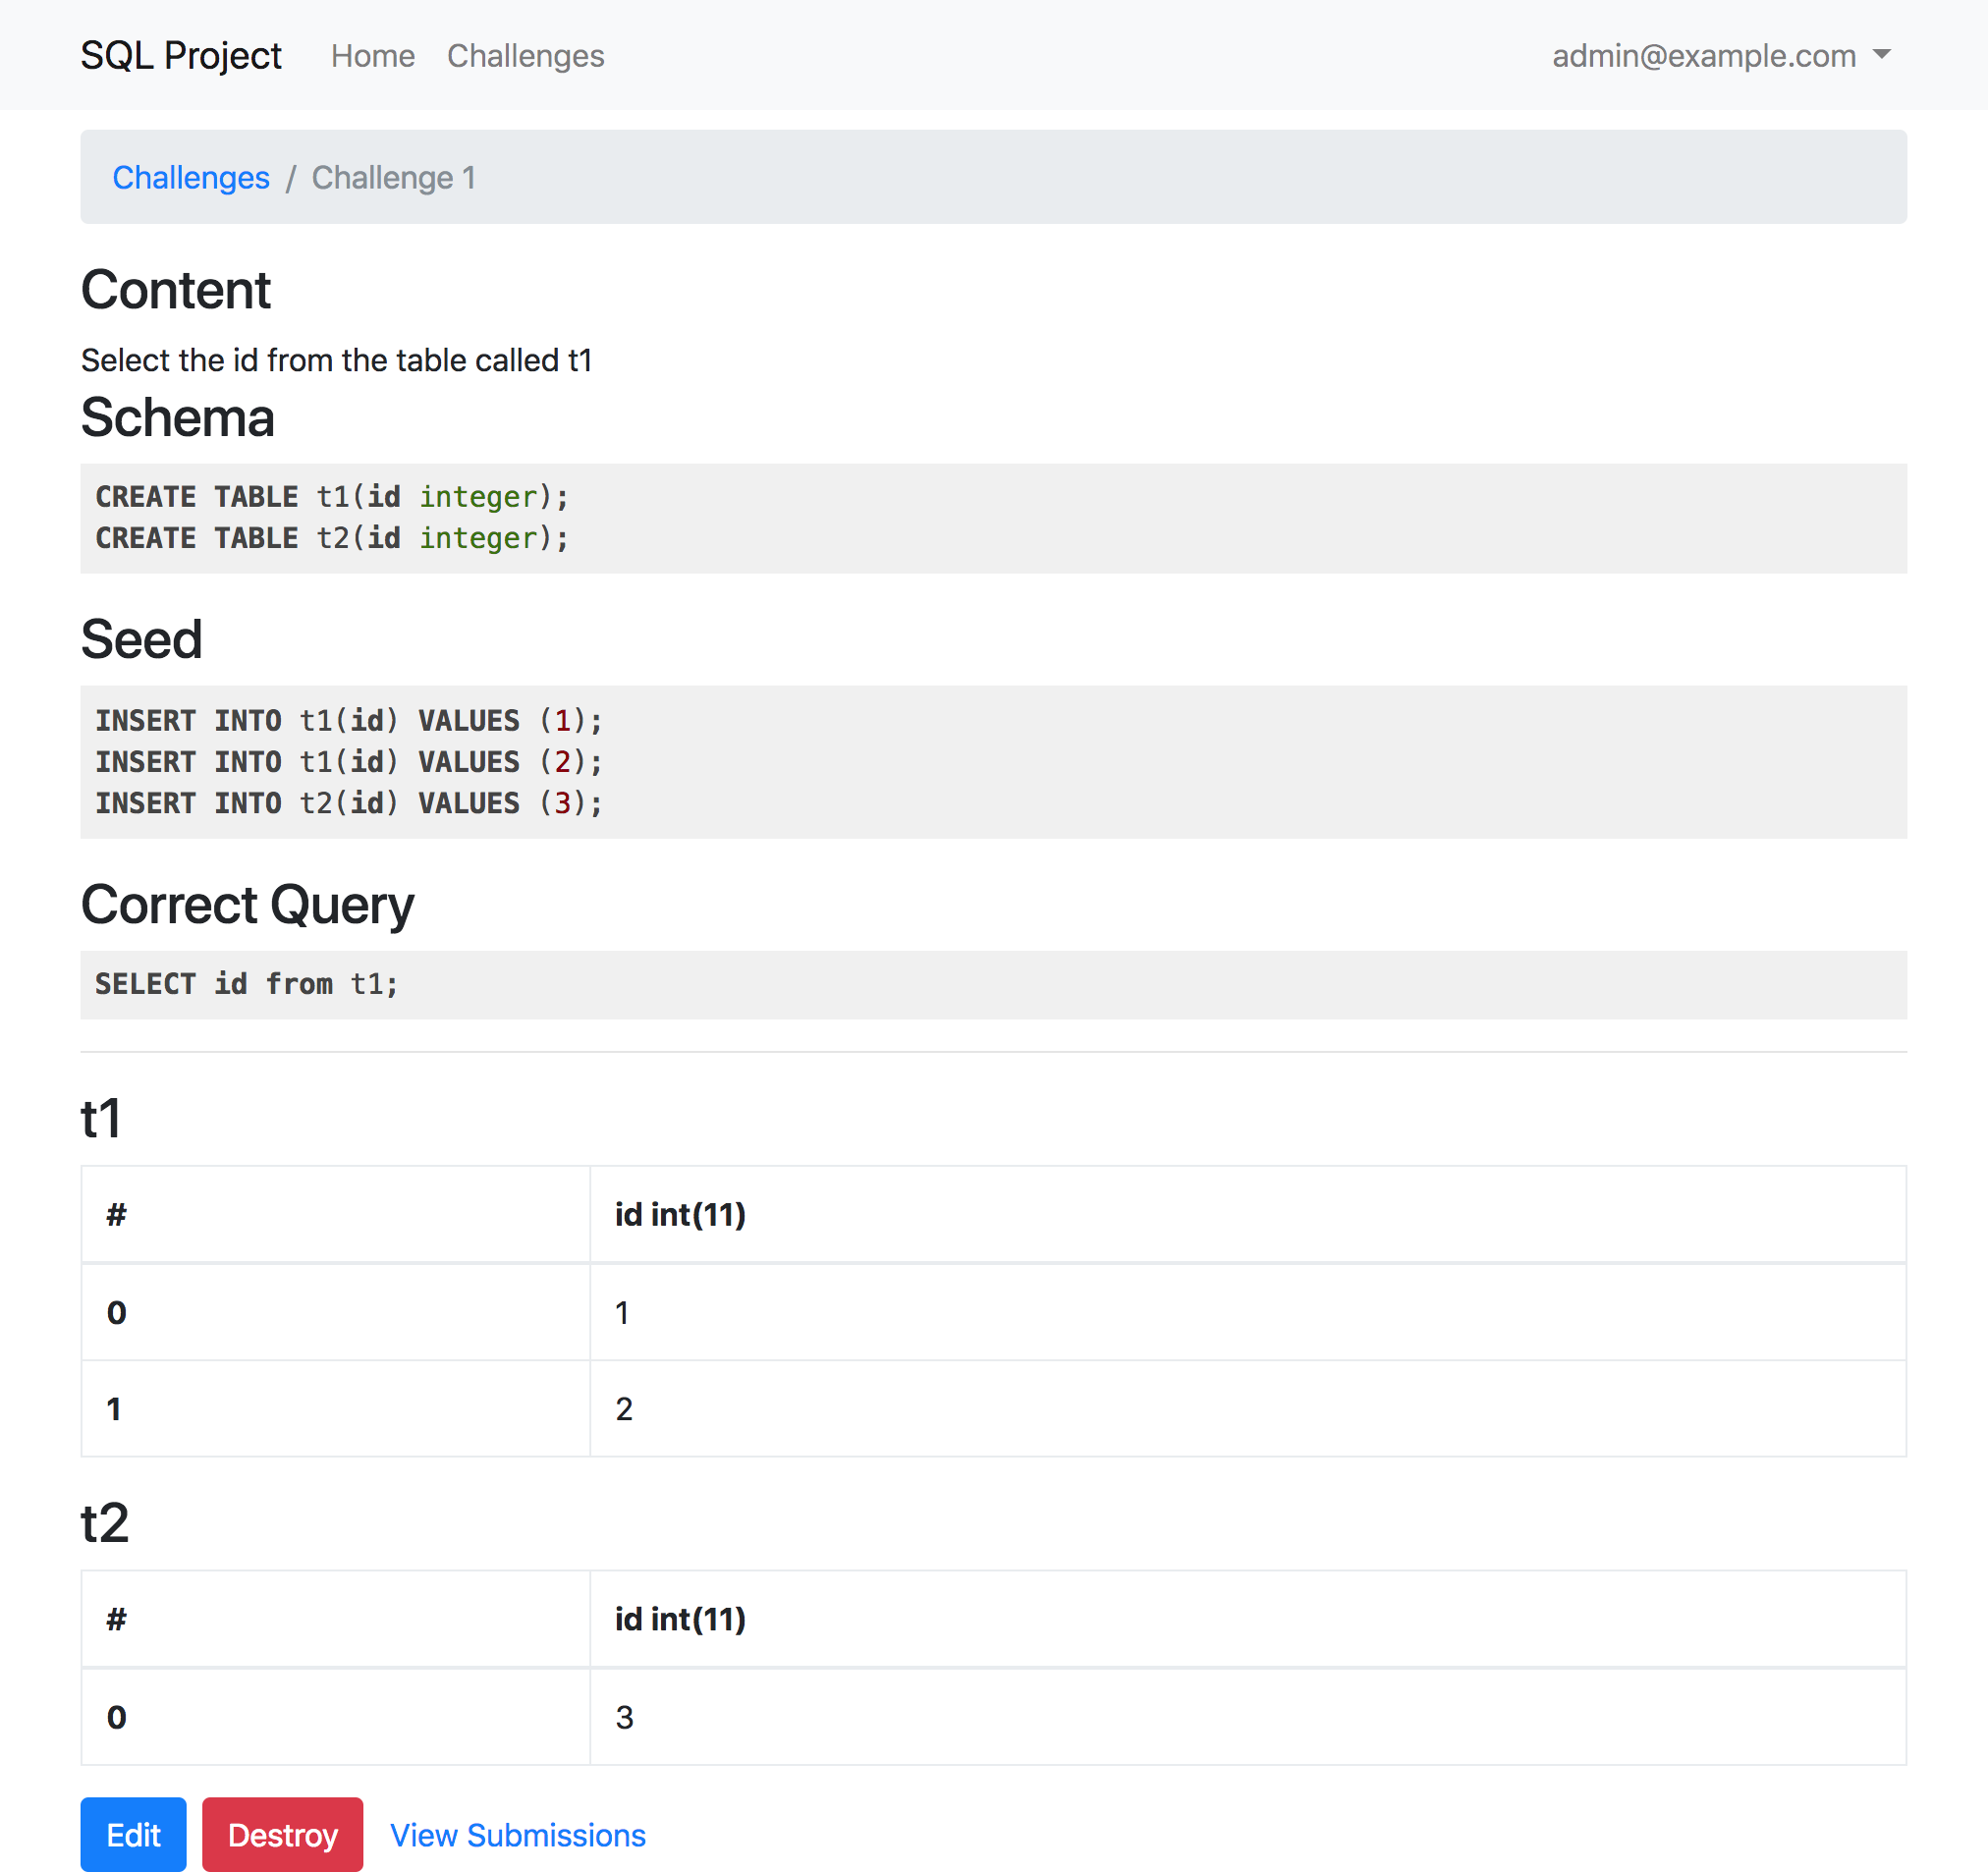
\includegraphics[width=\textwidth/4*3]{Appendices/adminchallenge.png}
    \caption{Admin's view of a new challenge}
    \label{fig:app:challengeadmin}
\end{figure}

An admin can then edit any challenge by clicking the edit button at the bottom of the page \ref{fig:app:challengeadmin}. The edit page is very similar to the creation form (\ref{fig:app:new_challenge}).

An admin can also delete a challenge by clicking the Destroy button at the bottom of the page \ref{fig:app:challengeadmin}.

\section{Submissions: student's view}

A student can submit a solution by first going to the \textit{New submission page}. To go to that page, he first needs to visit the challenges page (from the navigation bar), and then click the \textit{New submission} link for the desired challenge. The instructions are presented in figure \ref{fig:app:new_submission}.

\begin{figure}[ht]
    \centering
    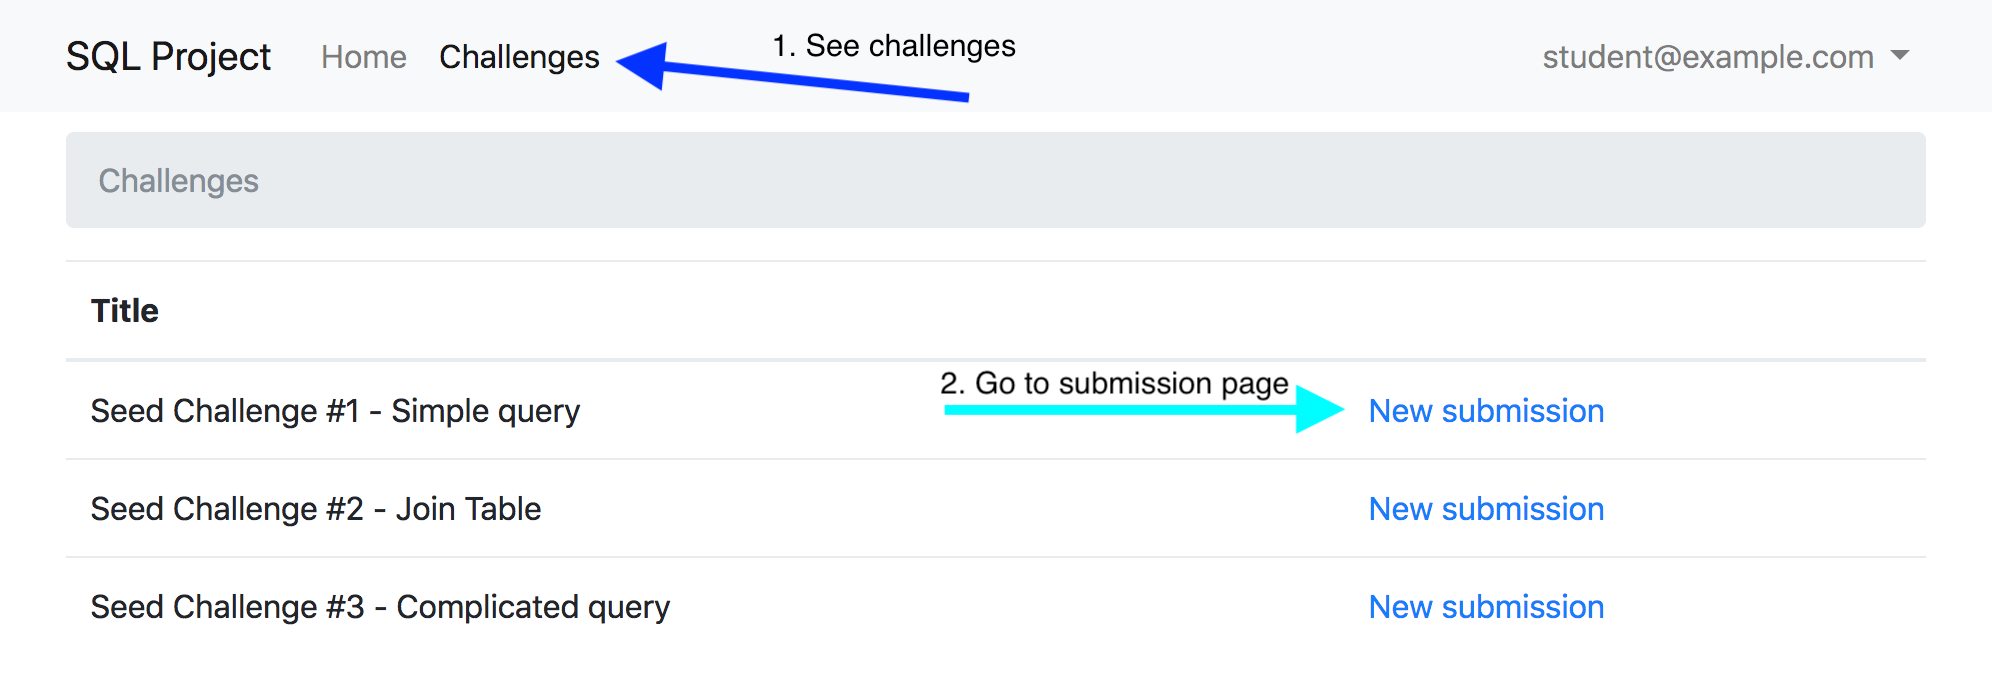
\includegraphics[width=\textwidth/4*3]{Appendices/challengeinde.png}
    \caption{Going to new submission page}
    \label{fig:app:new_submission}
\end{figure}

Once the user gets to that page, he will be able to see the schema of the database, both in the SQL form and in a tabular form. Here he can type the solution to the query. Figure \ref{fig:app:submit} presents this screen.

\begin{figure}[ht]
    \centering
    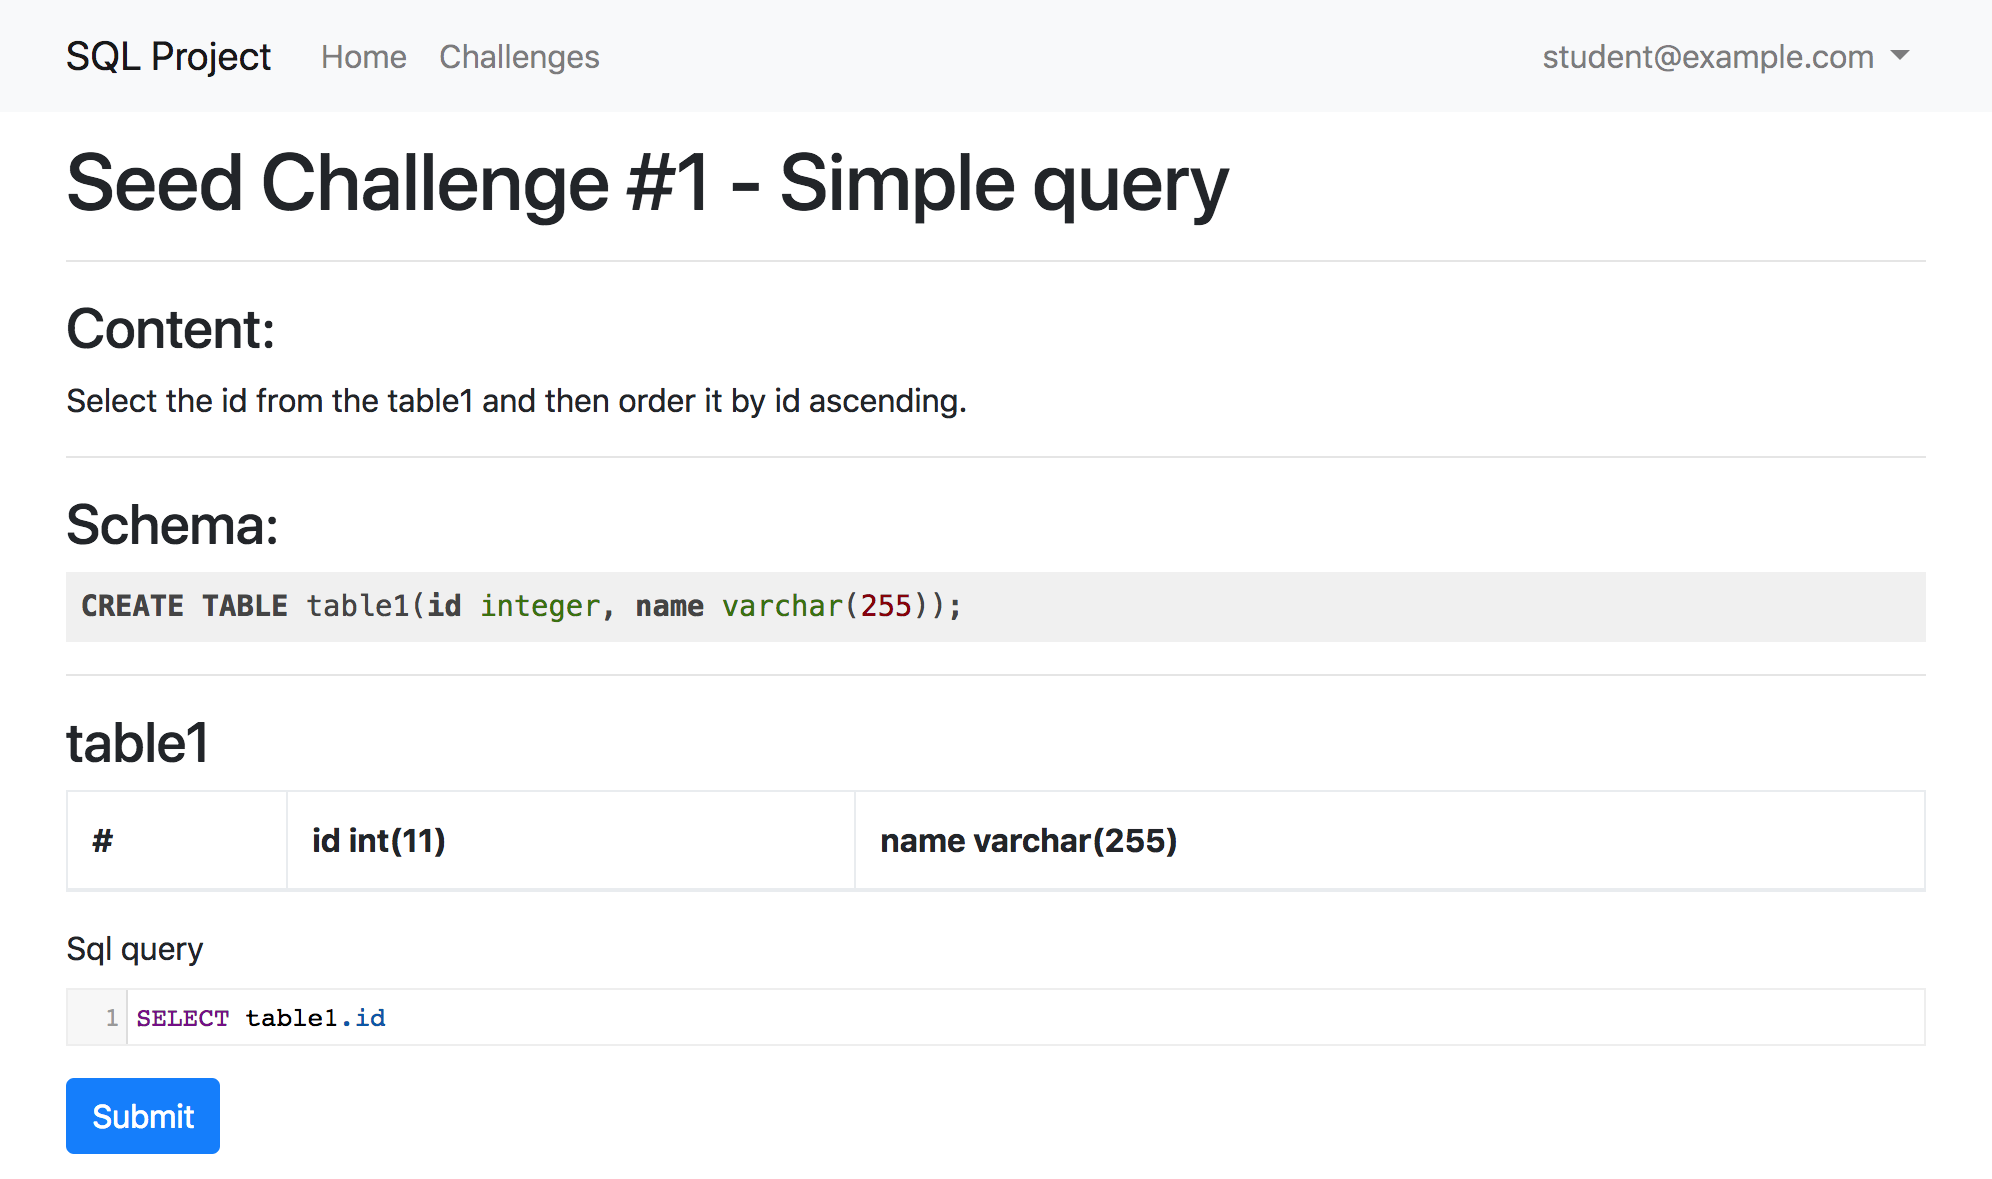
\includegraphics[width=\textwidth/4*3]{Appendices/submit.png}
    \caption{Submit solution page}
    \label{fig:app:submit}
\end{figure}

By clicking the Submit button on the page, the student will be able to see the results of the submission. If the query submitted has SQL errors, the user will see the errors on the same page (example in figure \ref{fig:app:submit_errors}.

\begin{figure}
    \centering
    
\includegraphics[width=\textwidth/4*3]{Appendices/submit_errors.png}
    \caption{Submit errors}
    \label{fig:app:submit_errors}
\end{figure}

If the compilation is successful, the user will either see a success message if the query is correct (figure \ref{fig:app:submit_correct}), or a hint if it's incorrect (figure \ref{fig:app:submit_incorrect}).

\begin{figure}[H]
    \centering
    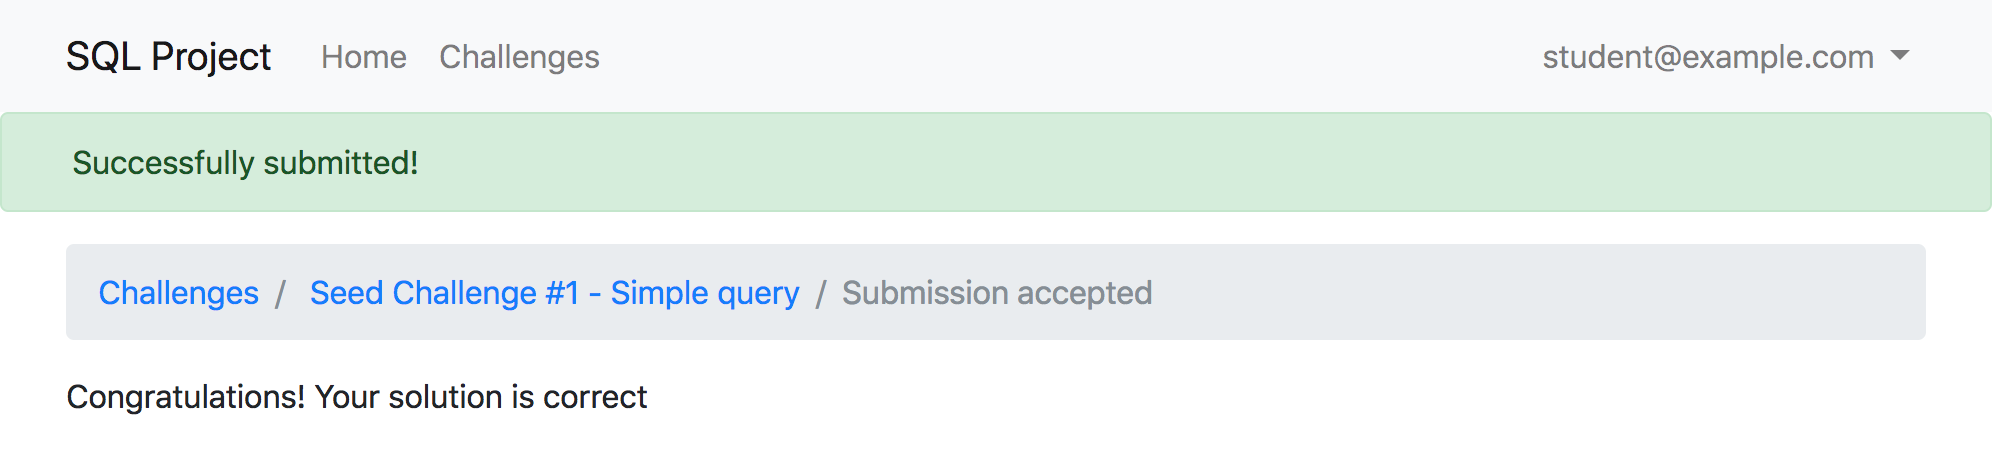
\includegraphics[width=\textwidth/4*3]{Appendices/submit_correct.png}
    \caption{Submission message for correct query}
    \label{fig:app:submit_correct}
\end{figure}

\begin{figure}[H]
    \centering
    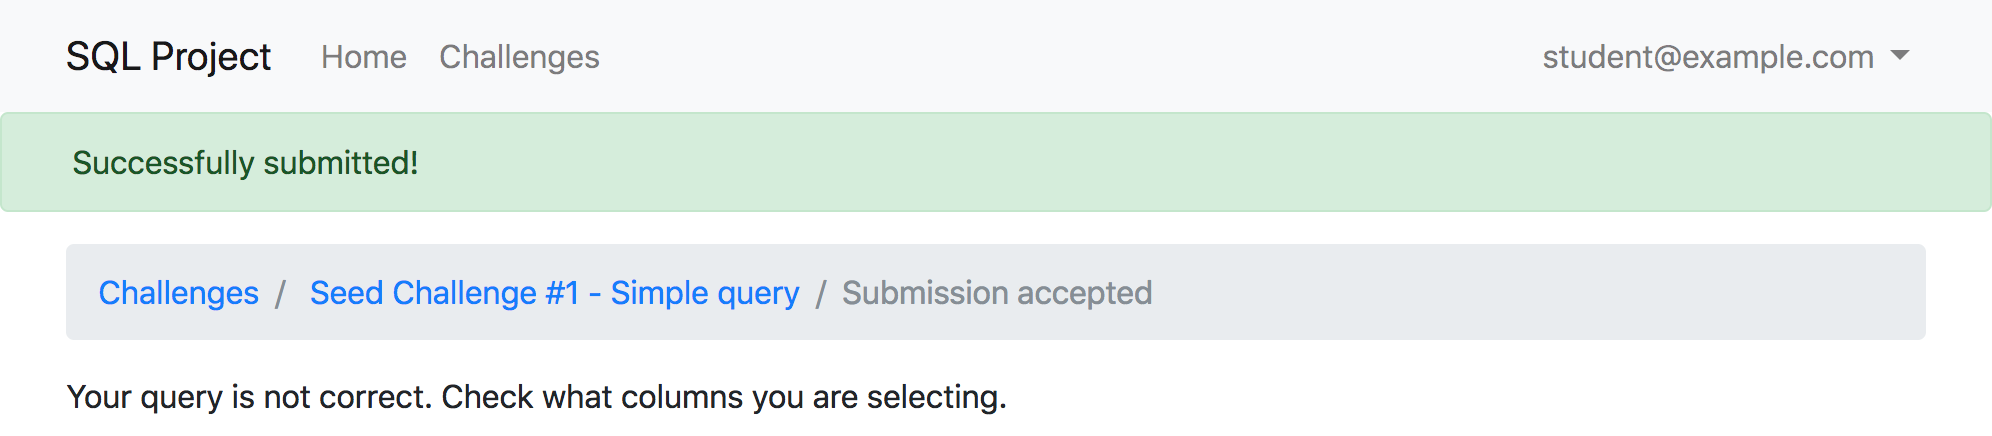
\includegraphics[width=\textwidth/4*3]{Appendices/submit_hint.png}
    \caption{Submission message for correct query}
    \label{fig:app:submit_incorrect}
\end{figure}

\section{Submissions: instructor's view}

To view student's submissions for a challenge, the instructor must click the link "View submissions" from the challenge page (presented in \ref{fig:app:challengeadmin}). The submissions page will include all submissions for a challenge. The page is presented in figure \ref{fig:app:submissions}.

\begin{figure}[ht]
    \centering
    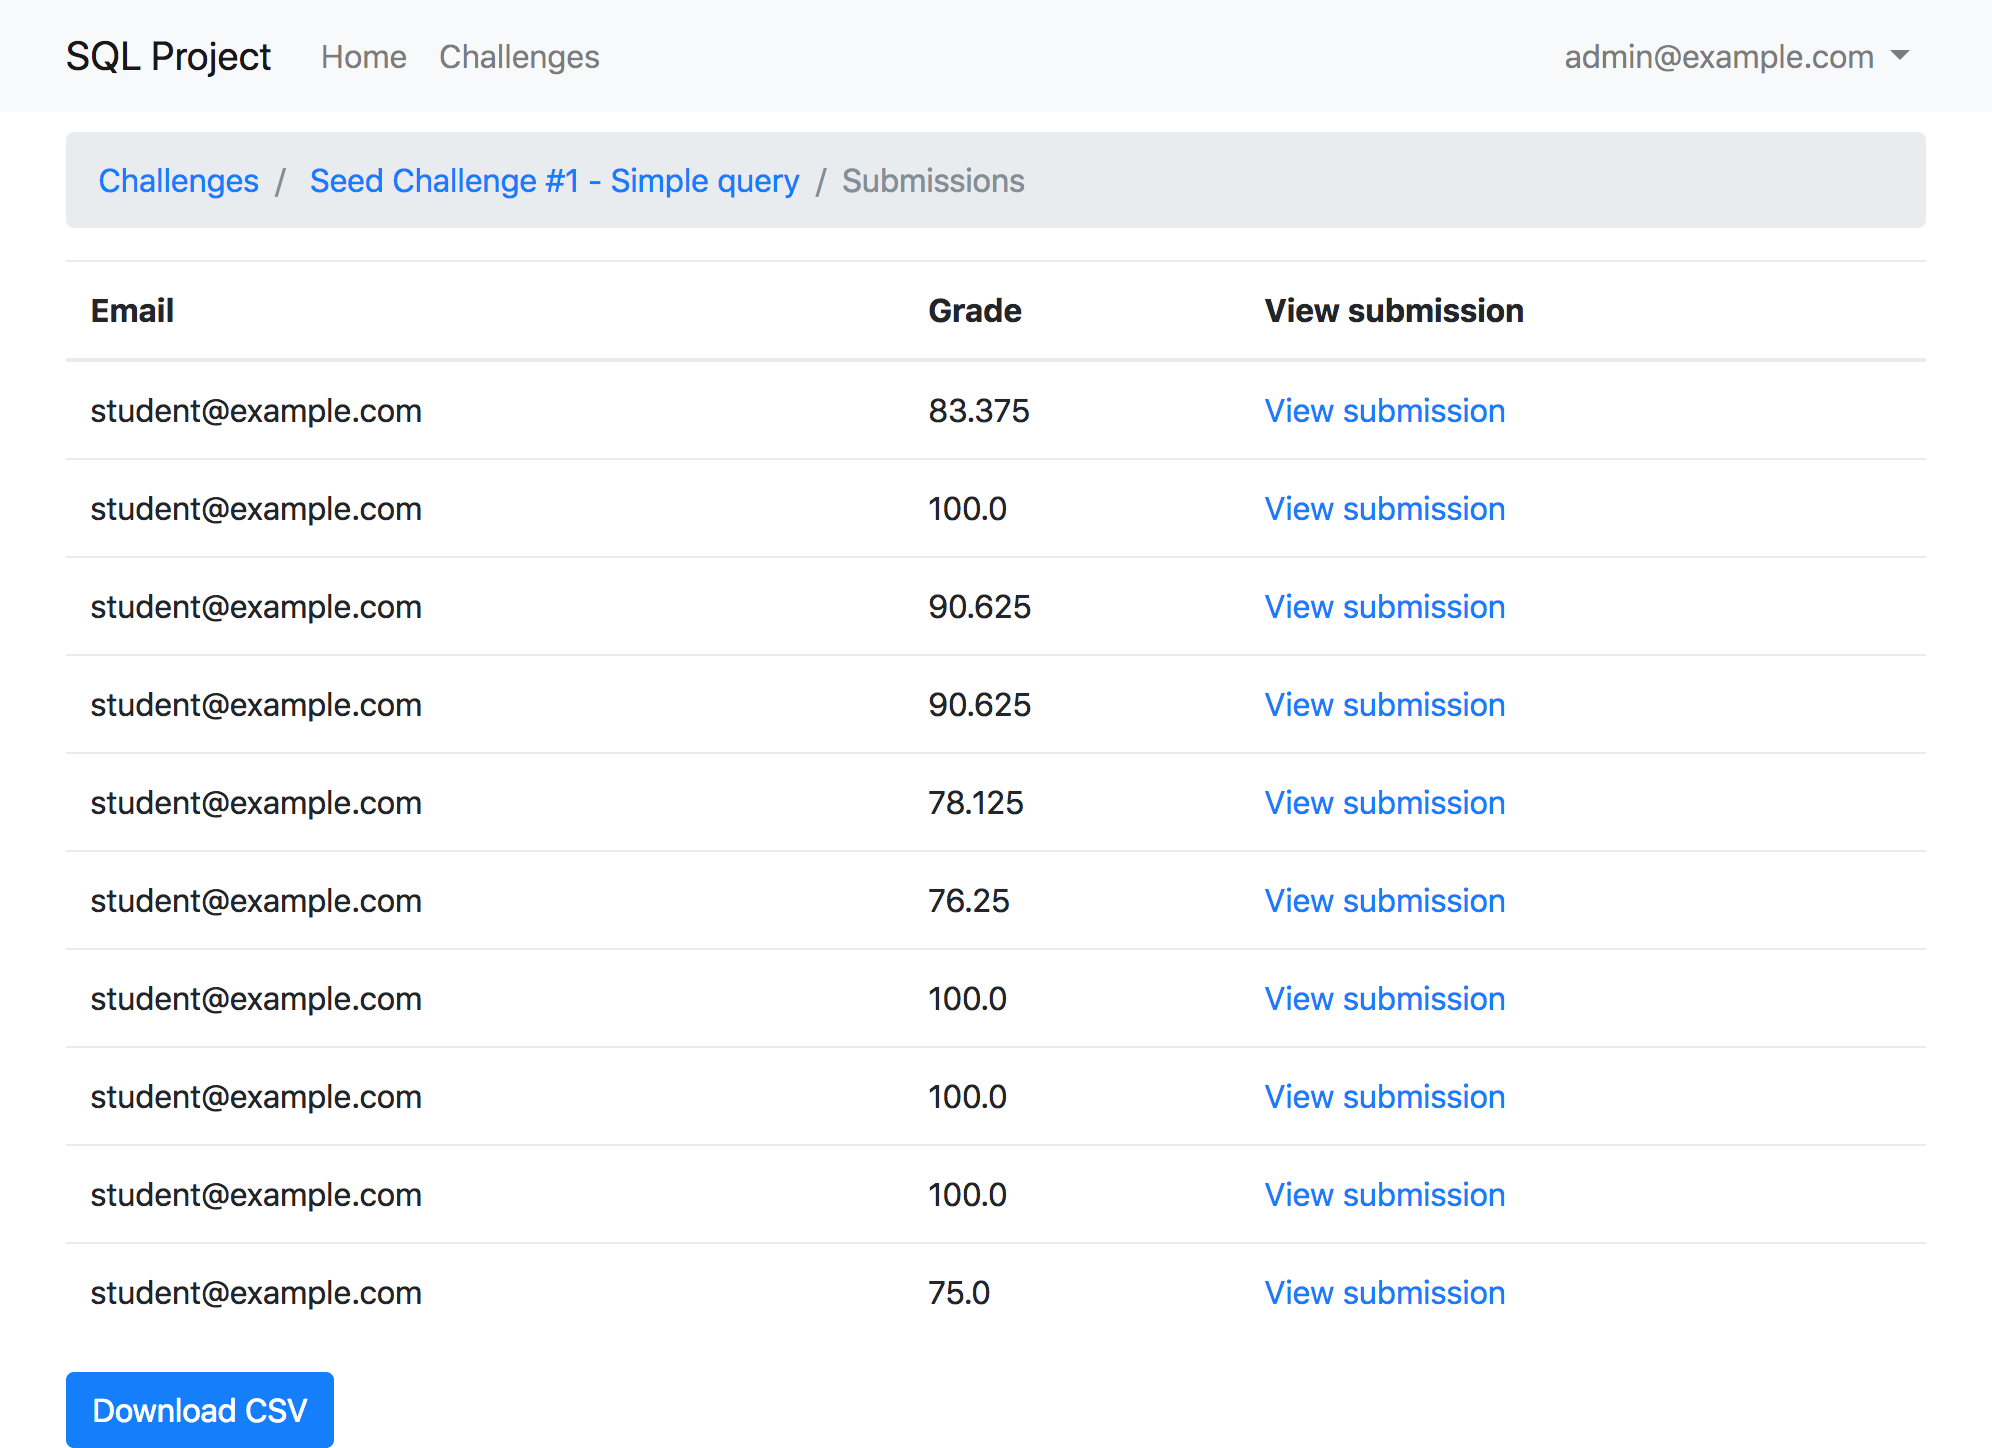
\includegraphics[width=\textwidth/4*3]{Appendices/submissions.png}
    \caption{Submissions for a challenge}
    \label{fig:app:submissions}
\end{figure}

At the bottom of the page there is a Download CSV link that will download a CSV containing the best result for each student.

A instructor can see more details about a submission by clicking the View submission link. The new page will include all details about a submission. An example of such a page is included in figure \ref{fig:app:submission_report}.

\begin{figure}
    \centering
    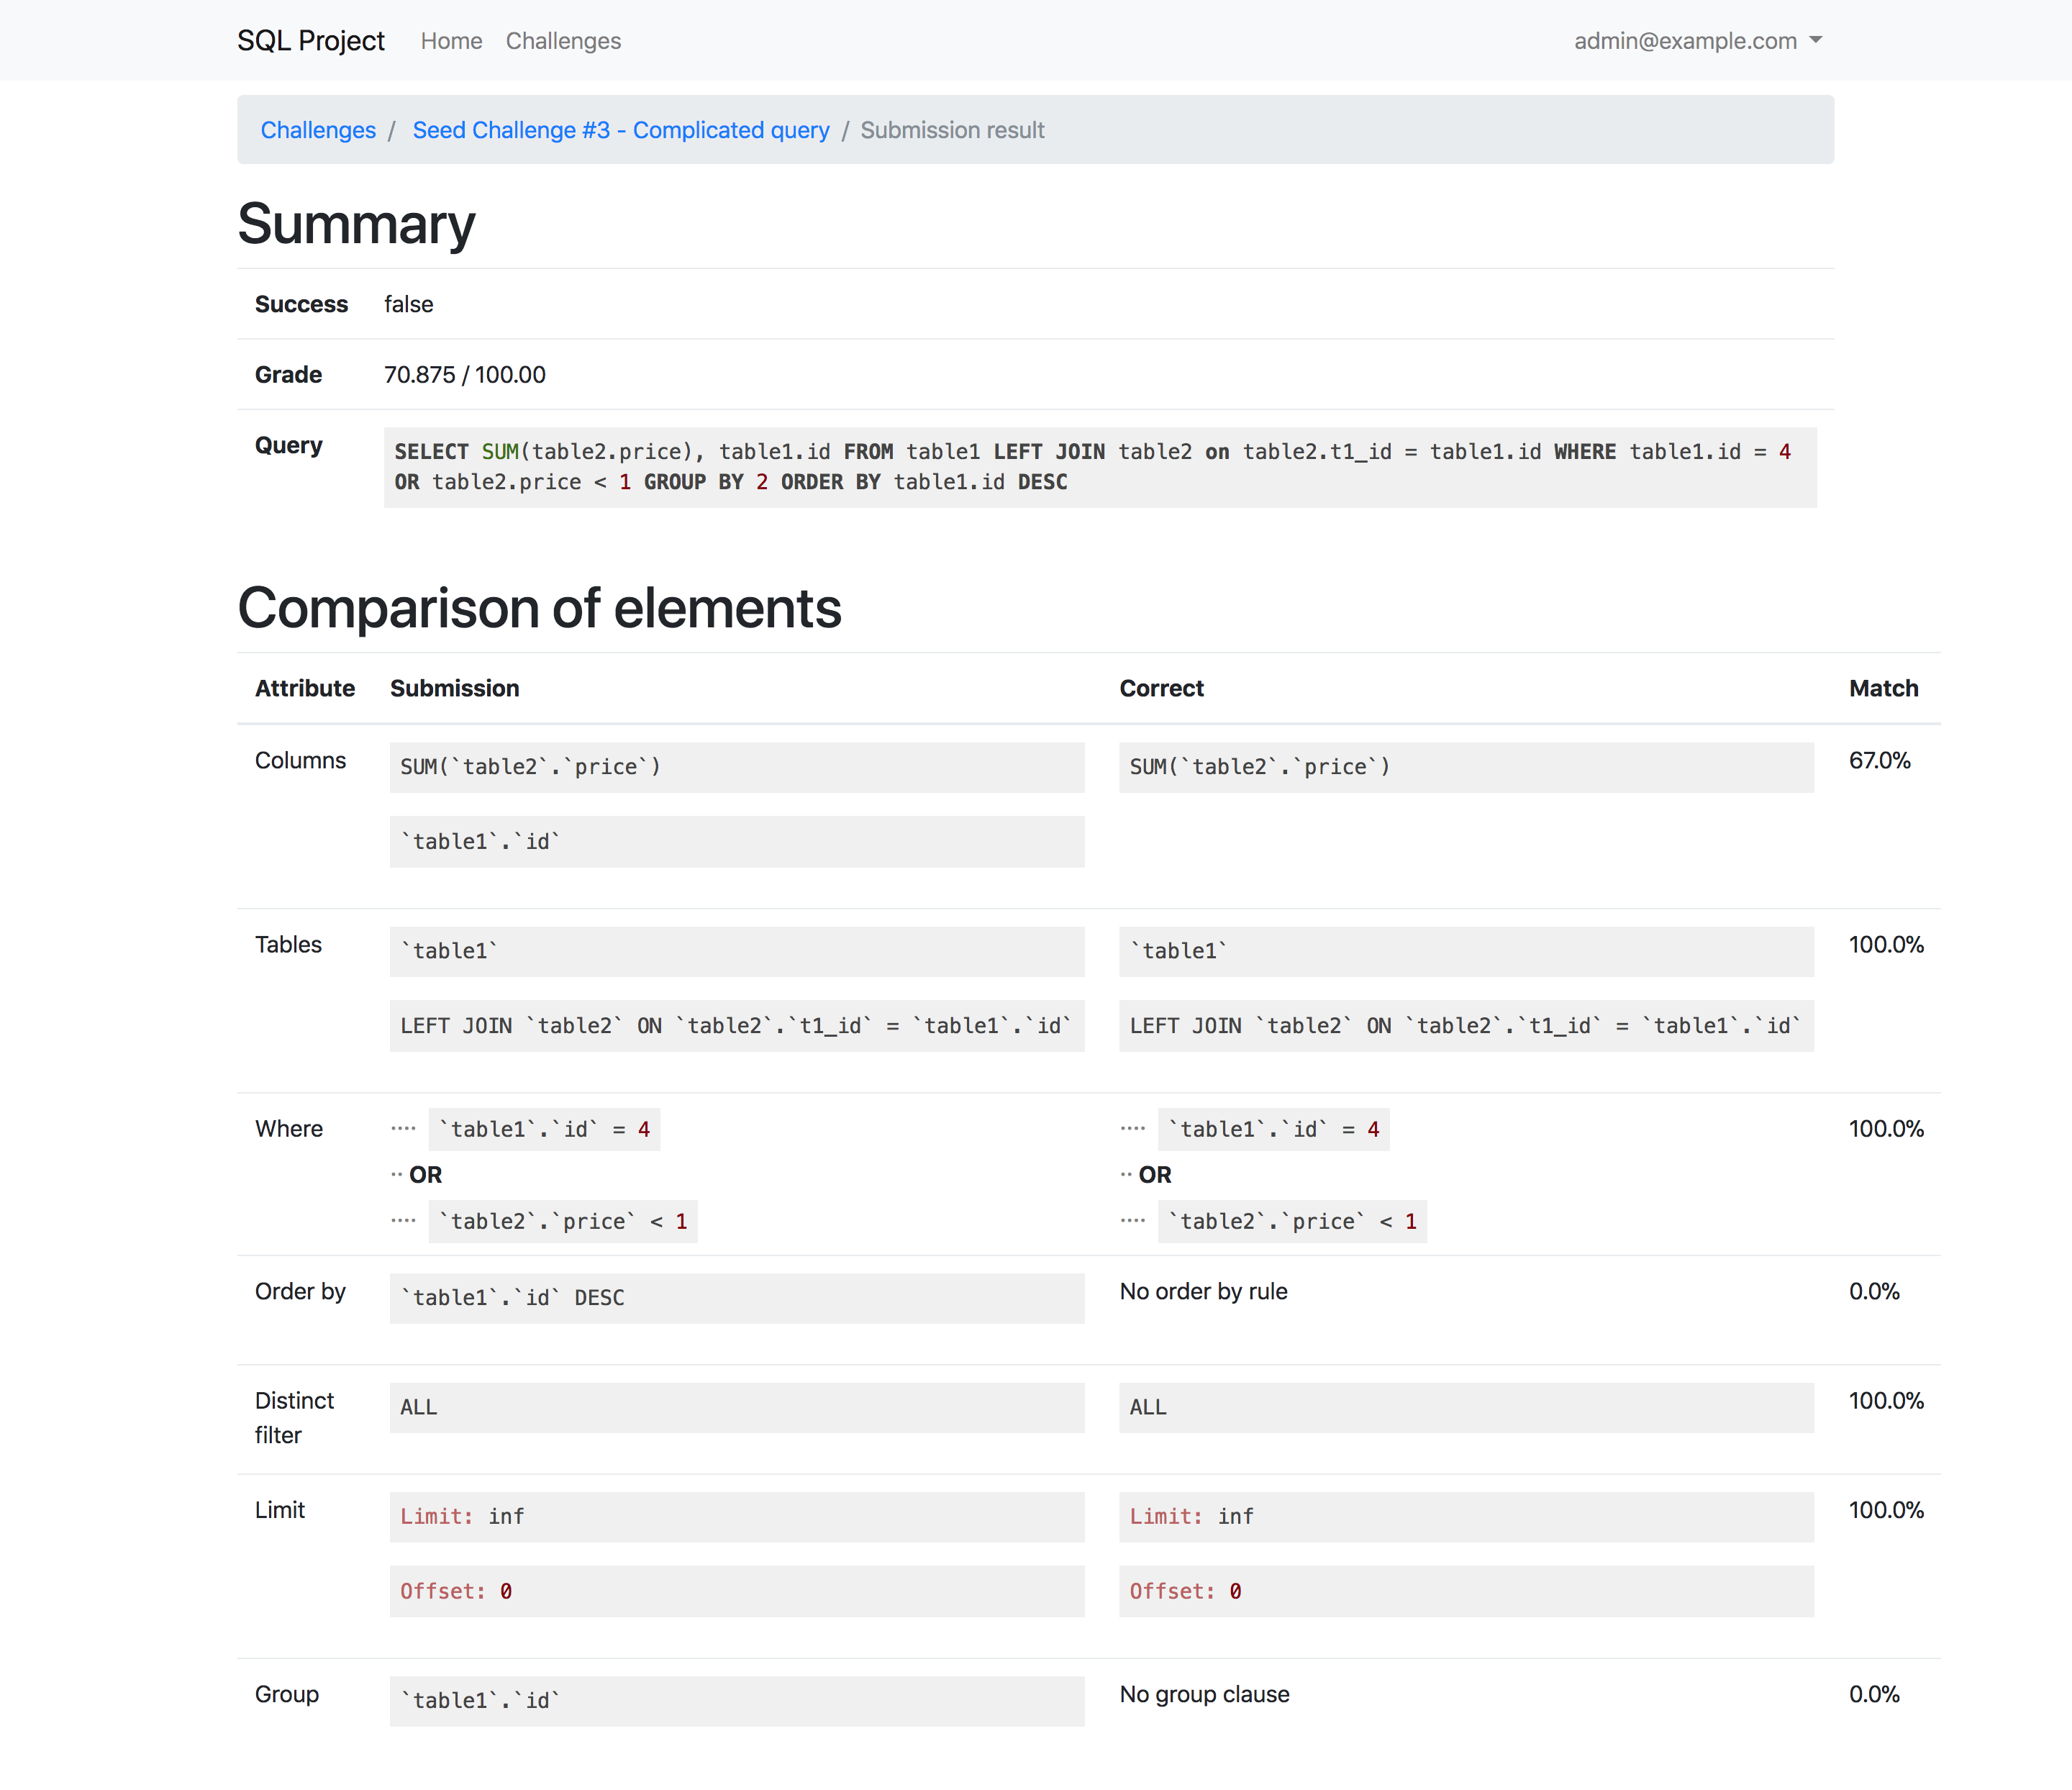
\includegraphics[width=\textwidth/4*3]{Appendices/submission_report.png}
    \caption{Caption}
    \label{fig:app:submission_report}
\end{figure}